\documentclass[11pt]{article}
\usepackage{amsmath}
\usepackage{graphicx}
\usepackage{float}
\usepackage{blindtext}
\usepackage{subcaption}
\usepackage[a4paper,margin=2cm]{geometry}
\usepackage{fancyhdr}
\usepackage{longtable}
\usepackage[
    backend=biber,
    style=ieee
]{biblatex}
\usepackage{xcolor}
\usepackage{soul}
\usepackage{listings}

\newcommand{\hlc}[2][yellow]{{%
    \colorlet{foo}{#1}%
    \sethlcolor{foo}\hl{#2}}%
}


\addbibresource{report.bib}

\graphicspath{ {./images/} }

\pagestyle{fancy}
\fancyhead[C]{Report}
\fancyhead[L]{EEE3027 Calculator Assignment}
\fancyhead[R]{2nd of May}

\cfoot{} % get rid of the page number 
\fancyfoot[L]{6596386}
\fancyhead[C]{}
\fancyfoot[R]{\thepage}

\begin{document}
\begin{titlepage}
    \begin{center}
    
\includegraphics[width=\textwidth]{Logo.png} % also works with logo.pdf
    \vfill
    \Huge
    \textbf{EEE3027: Calculator Assignment}
    \vfill
    \huge
    Assignment Report\\
    \vspace{1cm}
    \Large
    2nd of May 2023\\
    URN: 6596386\\
    \vfill
    \vfill
    \Large
    Department of Electronic Engineering\\
    Faculty of Engineering and Physical Sciences\\
    University of Surrey\\
    \end{center}
\end{titlepage}

\begin{abstract}
This report covers the work done on creating and testing an FPGA Calculator in VHDL as part of EEE3027 Digital Design with VHDL.
VHDL was used to program an FPGA capable of taking serial input,
converting the serial input to numbers and operations,
calculating the result,
converting the result back into serial, 
and finally transmitting the result back.
The final design allows for a user to input, over serial, any integer between -32767 and 32767 (a signed 16-bit value) with the following integer operation : addition, subtraction, multiplication, and division. 
The FPGA will then return the result if it can be represented as a signed 16-bit value, otherwise it will return an error. 
The report also covers background theory for UART communication, an exploration of the original provided code, and a discussion on timing and physical implementation on a Minized Zynq board.
\vspace{1cm}
\end{abstract}
\tableofcontents
\pagebreak

\section{Overview}

The objectives of this assignment were to create an arithmetic calculator using the std.numeric library and provided UART code.
This provided code first has to be debugged and tested.
The calculators basic requirement was to compute values given in the "$A {+-*/} B$" format, with no specific instructions of the range of values of $A$, $B$ or the output.
For the implementation created for this assignment the calculator is able to take inputs and provide outputs that can be described as signed 16-bit integers (ie between -32767 and 32767),
however, through the use of generics this range can be changed.
The serial UART input is then processed into the two expected numbers and operations, with any character that is not a numeral (0 to 9) or an operator character ($+-*/$) being ignored.
At the end of the input a carriage return character (ASCII Hex code $0D$) is required to indicate the end of number $B$.
A carriage return is also transmitted at the end of the calculator response with the result.
Furthermore the final design will output a special character, "!", when an operation is invalid (such as dividing by zero) or the output is outside the calculators range.

\begin{figure}[H]        
    \centering
    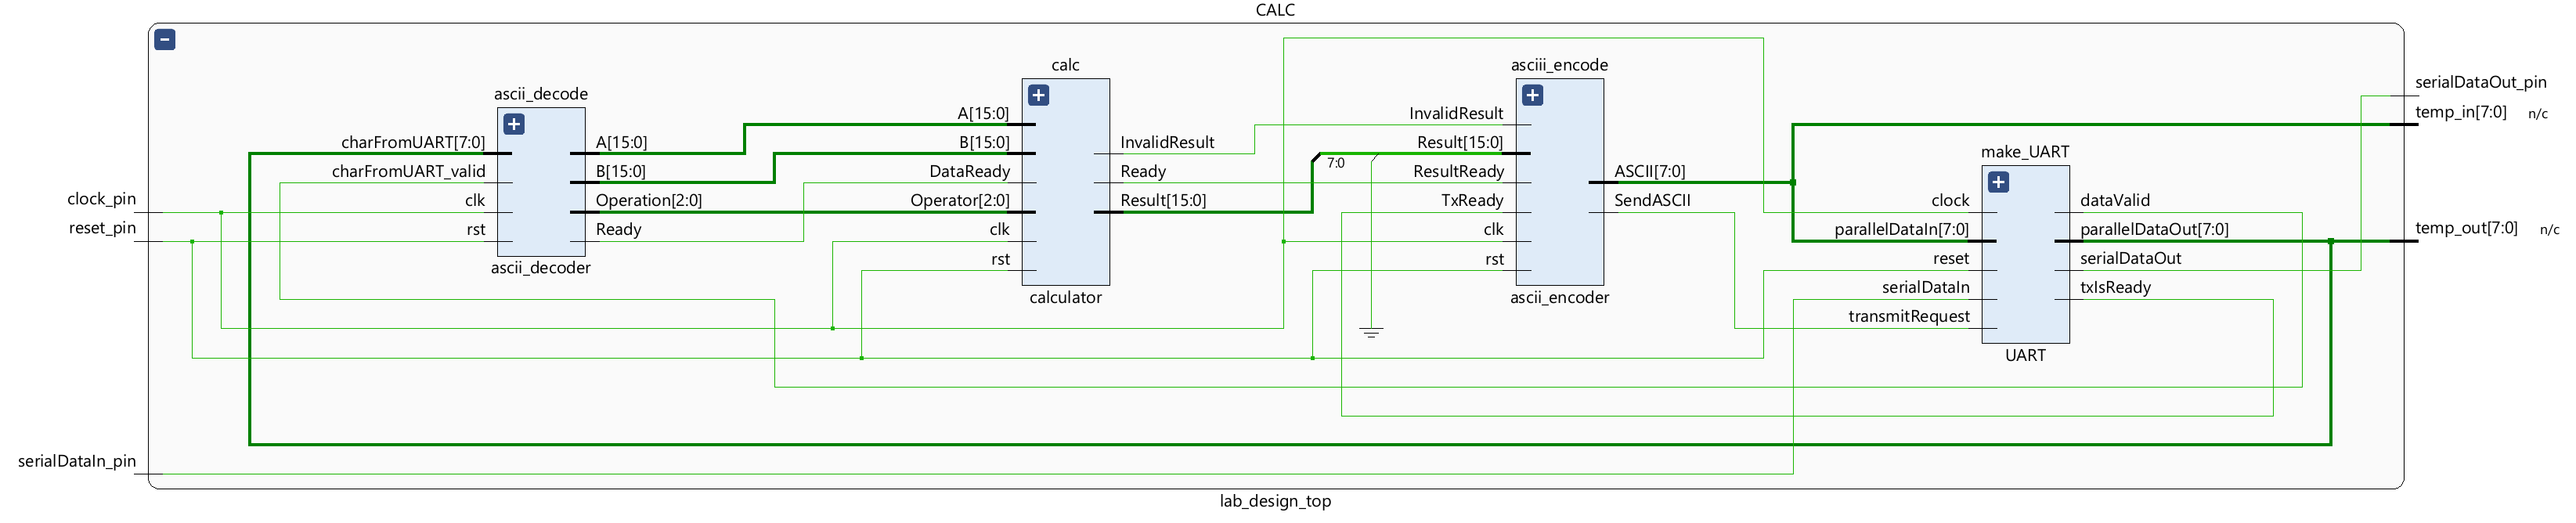
\includegraphics[width=\textwidth]{TopLevelImp.png}
    \caption{Top Level Implementation of Calculator}
    \label{fig:toplevel}
\end{figure} 

To achieve this functionality the design seen in figure \ref{fig:toplevel} was created, with four main components all interacting together.
These components are the UART block, the ASCII decoder, the calculator, ASCII encoder.
The UART block handles the receiving of serial UART data and converting it to parallel data as well as taking parallel data and sending it as serial UART.
The ASCII decoder takes the parallel data, assuming they are ASCII codes, and converts into two numbers and a operation.
The calculator computes operations between two numbers, the provides a result as well as a signal if the operation is invalid.
THe ASCII encoder takes a result, as well the invalid signal, and converts them into a sequences of parallel ASCII codes that it sends to the UART block.
Details on the design and operation of all of these components, as well information on testbenches and implementation on a Minized Zynq FPGA board are provided in


\section{UART}
\subsection{UART Theory}
UART stands for universal asynchronous receiver-transmitter and is a very common device-to-to device communication protocol\cite{UART}.
For this assignment a two-way UART connection is utilized,
allowing two devices (the FPGA and a connected PC) to transfer data between each other regardless of clock rate as long as they communicate over a predefined rate know as the baud rate.
Unlike other communication protocols such as SPI or I2C, UART only ever has one "master" device and one "slave" device a third device cannot be added on the same lines.

UART takes parallel data and converts it into a bit by bit frame to send.
The frame always start with the start bit, which takes the line low for one cycle as UART is normally high.
then each data bit is sent one by one (least significant bit first) with a 1 being high and a zero being low.
Some implementation will include a parity bit after the data, which will be 0 if the data total is odd and 1 is the total is even.
Parity is useful to ensure that data been altered during transmission, which can occur due to "electromagnetic radiation, mismatched baud rates, or long-distance data transfers"\cite{UART}.
The provided UART however does not utilize the parity bit.
At the end of the message a stop bit is sent going from low to high.
Equation \ref{eq:uart_sample} shows an example of how data gets converted to 

\begin{align*}
    \text{Data} &= 01000001
    \stepcounter{equation}\tag{\theequation}\label{eq:uart_sample} \\
    \text{UART Frame} &=    \overset{\text{Start Bit}}{\{0\}}
                            \underset{\text{Data}}{\{1000 0010\}}
                            \overset{\text{Stop Bit}}{\{1\}}\\
\end{align*}


The final key concept behind UART is the baud rate, which the number of signals per second.
In the case of UART baud rate represents how long each bit is held high or low.
As UART is asynchronous, each device needs to know baud rate ahead of time and generate its own clock at the baud rate.
This is enough to transmit UART as the line can simply be updated each clock cycle,
however for receiving the line needs to be checked more often as the devices baud clocks can be out of phase by half a period and because reals signal have non-instantaneous transition periods from high to low meaning that is best to check the signal in the middle of each cycle.
To do this there is a secondary oversampled clock, oven 16x, that is used in the receiver to check in the middle of each received by instead.
Then when a start bit is received the receiver will wait for roughly half a baud to sample the next bit.
After this point the the receiver will wait 16 of the oversampled rates to take the next sample.
Some implementations may take multiple samples around the midpoint to get a more accurate result, however this implementation takes only one measurement.
Once enough measurements have been made, something else that needs to be predefined, the receiver will wait for the stop bit.

% This method of having both receiver and transmitter create their own baud clock means that communication occurs without a shared clocked, letting devices running at vastly different frequencies communicate.
% Ideally when each device will perfectly generate a clock for baud allowing for flawless communication even when the receiver and transmitter are completly out of phase (ie half a baud period apart), however the baud rates a device can support are limited by its own clock.
% As the smallest unit of time a device can use is a clock period the actual baud rate may differ from the desired baud rate.
% For example with a 60 MHz clock the smallest unit is 16.66 ns, and to create a 115.2 kHz baudrate a 8680.56 ns period is required which can be approximated with 521 clock cycles (which is 8683.33 ns).
% This  means the acutal baudrate will be  115.207373 \cite{baudrate}

\subsection{UART Component}
\begin{figure}[H]        
    \centering
    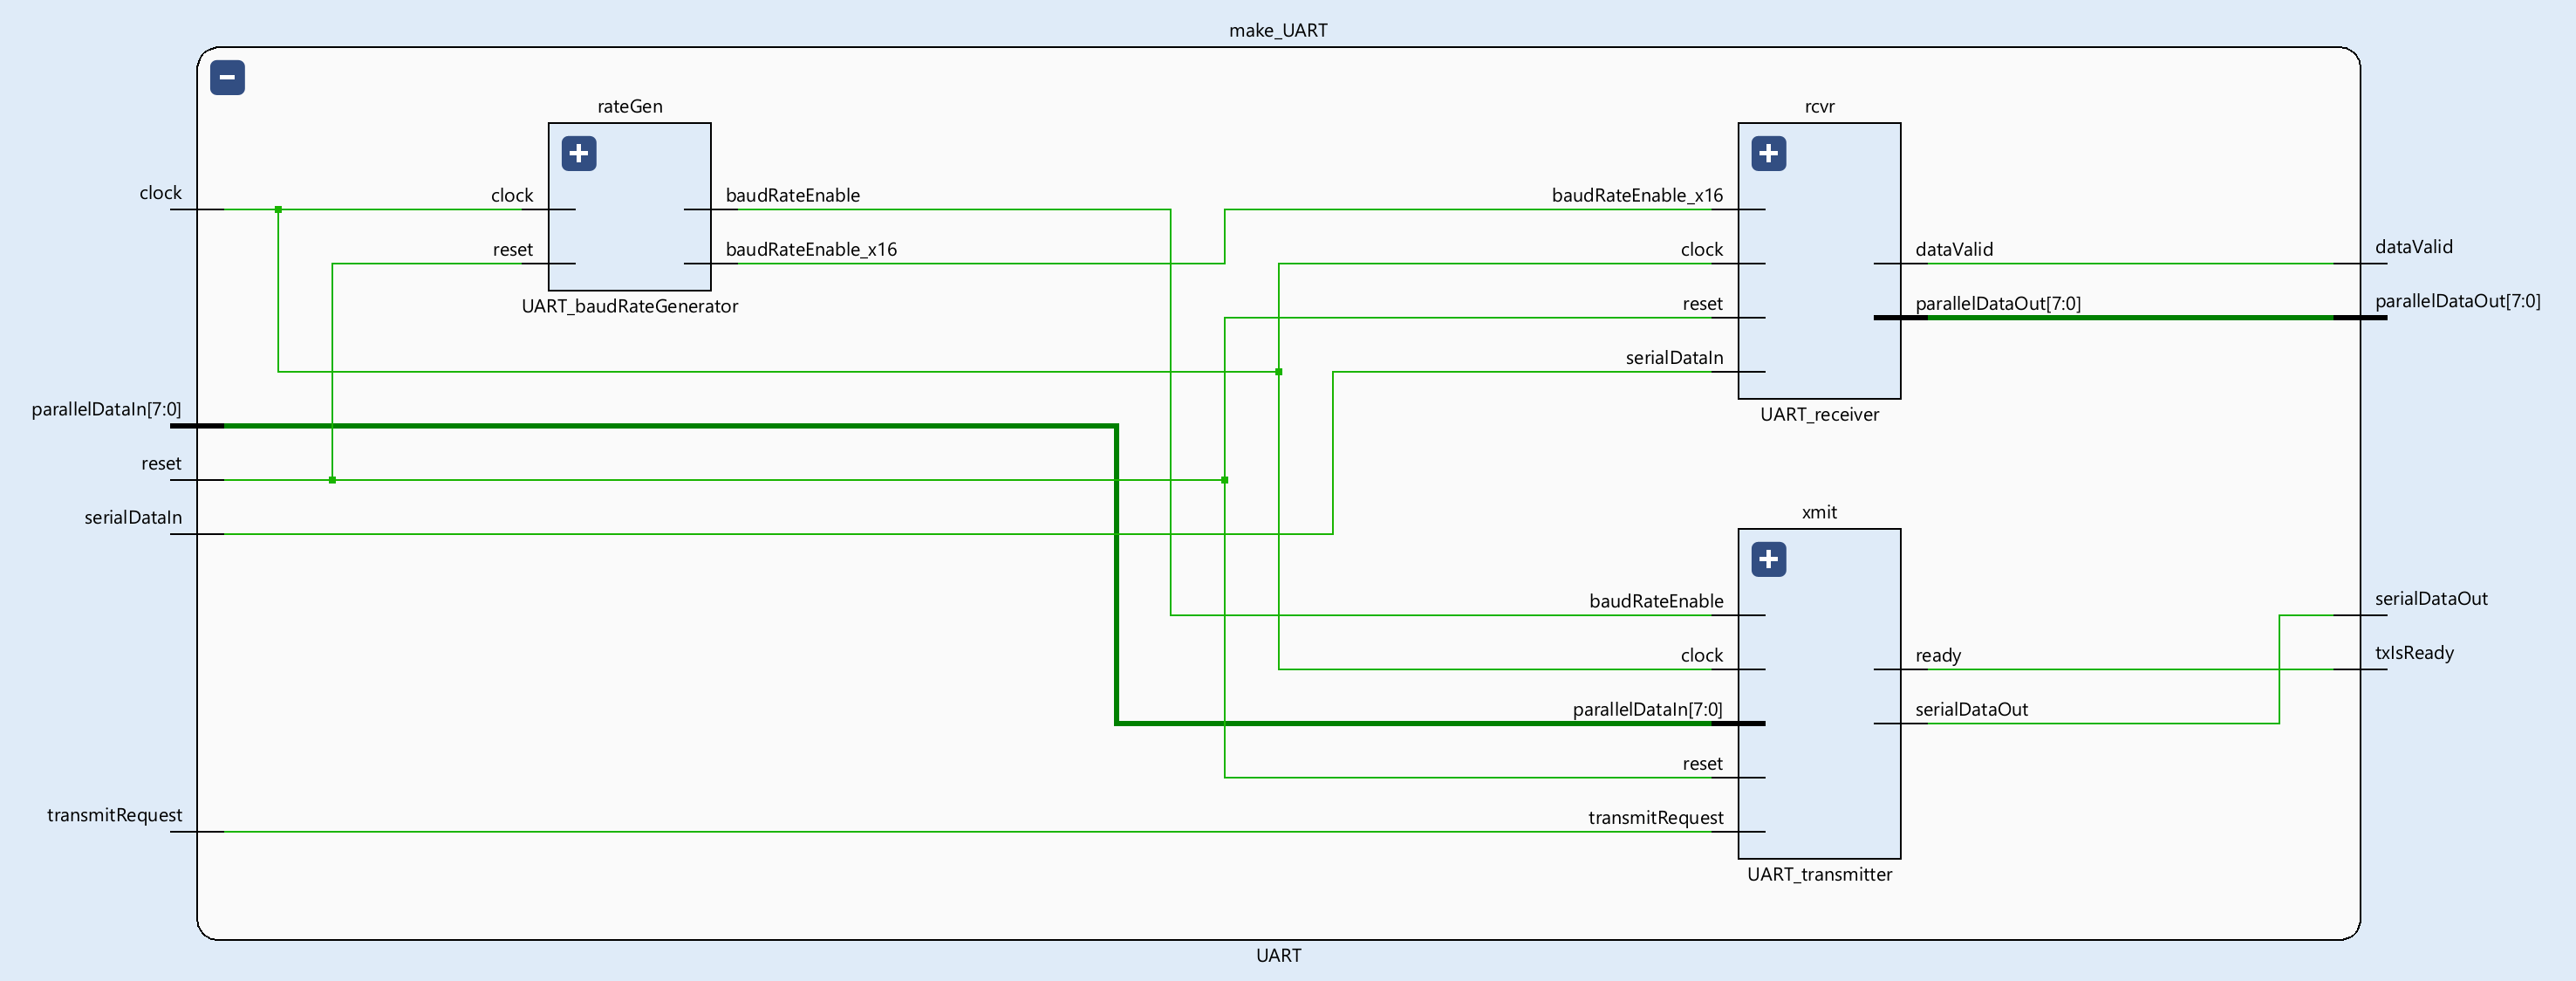
\includegraphics[width=\textwidth]{uartImp.png}
    \caption{UART Block Diagram}
    \label{fig:UARTimp}
\end{figure} 

Provided with the assignment was the VHDL code for a UART transmitter and receiver. 
This code required a few corrections to get in working order. 
The simpler of the fixes was that all files required the addition of the IEEE std\_logic\_1164 library. 
Testing also revealed that the UART receiver was not connected to the baudRateEnable\_x16 line which was quickly fixed in the port map.
The baud rate generator also had the incrementing of its baud counts moved with-in the if statements to avoid incrementing the variable and then instantly setting it to zero, in order to keep this from breaking the timing the check for completion was also altered.
With the fixes the components functioned as expected.

This means that the baud rate generator given a clock line and predefined with the clock frequency and desired baud rate will produce two outputs: a pulse at the baud rate and a pulse at 16 times the baud rate which connect to the transmitter and receiver respectively.
It does this by counting an the number of clock cycles and sending a pulse every x cycles and resetting the count, where x is the clock rate over the baud rate.
The baud rate transmitter takes five inputs, a clock, a reset, baud pulses, a transmit request and an 8-bit bus for the output date.
Every clock cycle it will check if the transmit request is high, once it is it will begin to send a UART message including start and stop bit containing the data that was on 8-bit bus when the transmits request was received.
This operation is achieved using a finite state machine, a diagram for which can be seen in figure \ref{fig:transmitsm}

\begin{figure}[H]        
    \centering
    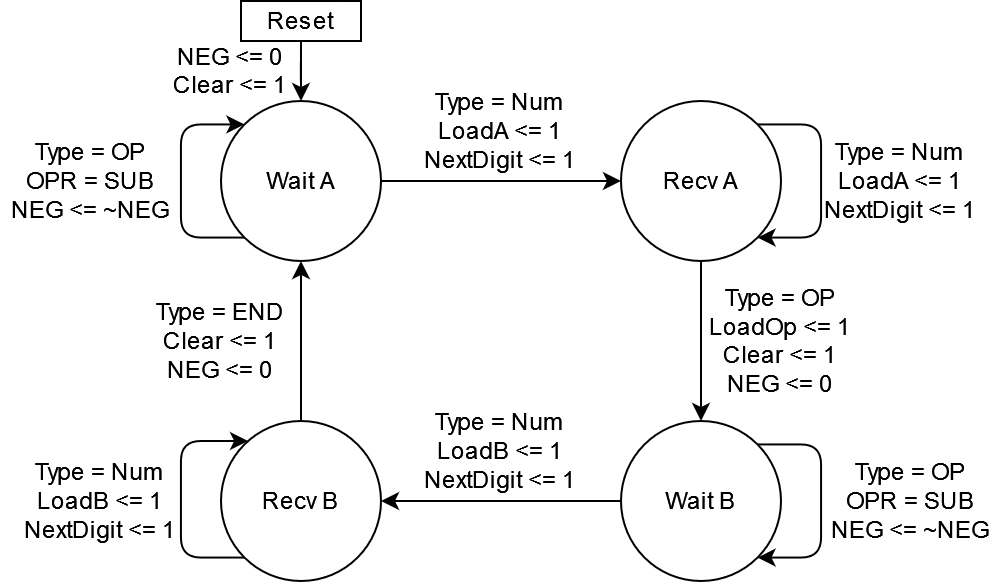
\includegraphics[width=.66\textwidth]{DecoderSM.drawio.png}
    \caption{UART Transmitter State Machine Diagram}
    \label{fig:transmitsm}
\end{figure} 

This diagram shows all the states, transitions and condition for transitions, as well as the outputs in those states and transitions. 
As the output depends both on the states and inputs, this is known as a Mealy state machine.
The $=$ sign indicates a conditions, with $<=$ being used when signals are set and $:=$ when variables are being set, this format will be used throughout the report.
Note that for this component the transition will occur only on the rising edge of baud pulses, not during the rising edge of clocks. 
The exception to this is the transmit request, which is monitored on clock rising edge and is essentially stored in a buffer as "go".
With the state machine the component will send out valid UART messages

The UART receiver takes in only a clock, a reset, and the oversampled baud pulses.
As an output it will give an 8-bit bus of data and a signal when the data is ready.
This operation is once more achieved with a state machine, seen in figure \ref{fig:receivesm}

\begin{figure}[H]        
    \centering
    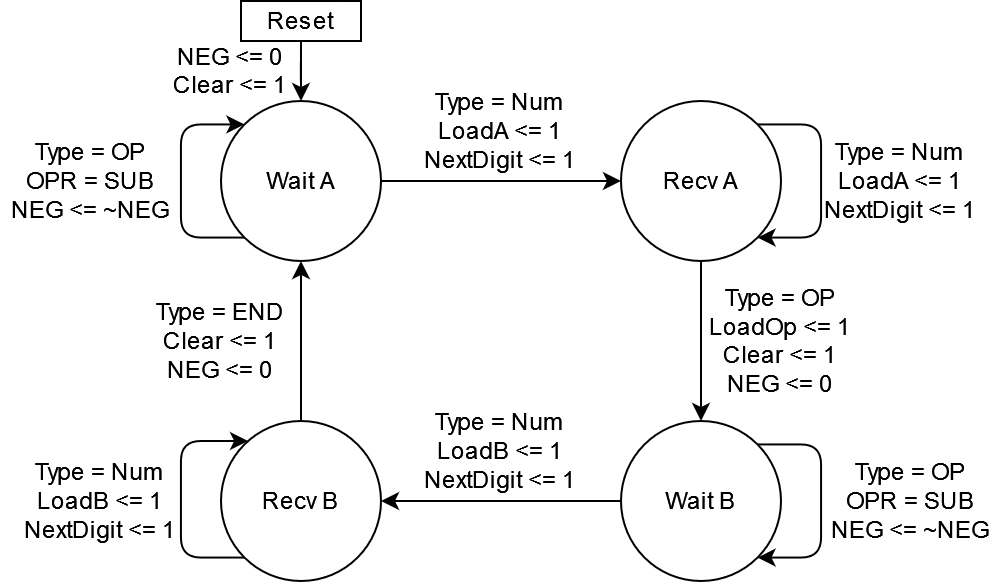
\includegraphics[width=.66\textwidth]{DecoderSM.drawio.png}
    \caption{UART Receiver State Machine Diagram}
    \label{fig:receivesm}
\end{figure} 

The core operation is similar, however as mentioned during the theory discussed the receiver makes use of a 16 times oversampled baud rate in order to take samples in the middle of data.
To achieve this the state machine transitions are triggered somewhat differently,
whenever the internal "countLoad" signal goes high the receiver will start counting up on a signal called "countValue" every oversampled baud rate and then often this count value will be used to govern what action the state machine takes next.

\subsection{Test Bench}
In order to test the UART module a simple test bench was created

\section{Original Design}
The original design, after correcting a few errors, did the following:

\section{UART Calculator}
This original design was heavily modified, with the original encoder being fully removed and the decoder being drastically changed, in order to meet the requirements for this assignment.
Figure \ref{fig:toplevel} shows this modified design.
As the UART components remains unchanged it will not be discussed again.
The overall design has three inputs: the clock, a reset line and the UART in, and only one output: the UART out.
Additionally there are four key generics: the clock rate, the baud rate, the maximum integer value, and the minimum integer value.
The first two values are used only by the UART component so that the baud pulses can be generated properly,
the integer range on the other will somewhat dynamically create version of the calculator cable of handling larger integers.
In practice the limit is -32767 to 32767, larger values may work in simulation but timing constraints prevent them from being implemented on physical hardware.


\subsection{ASCII Decoder}

% Upon receiving a UART message the receiver will send a ready signal as well as a parallel bus with the data,
% for this calculator it is assumed that these messages contain ASCII characters.
To do any calculating the inputted ASCII character, converted from serial to parallel in the receiver, need to be converted into two numbers, which will be referred to as A and B, and an operation.
This is done in the ASCII decoder which start by taking the incoming parallel data and "decoding" it.
THis is done in the decoder, which treats the parallel data as an unsigned integer and check wether the data is between the range of 48 to 71, the range of numerals 0 to 9.
If so the data outputs a signal labeling the message as a numeral (a custom type created for the calculator) and also output the numeral as an 4-bit numbers (by subtracting 48 from the incoming data).
Otherwise the decoder checks for operations, $+-*/$, which are ascii codes 43, 45, 42, and 57.
If these are detected a signal is output labeling the incoming data as an operator (the same custom type as before) as well as another custom type labeling the specific operator.
The final ASCII character that is checked for is number 13, which is carriage return.
For this design carriage return is used to signify the end of a message.
With any valid message the decoder will also output a character ready signal for the state machine.
If the message is any other value it is simply ignored meaning that an inputs of $-AB1cs 2 + 3 hh4$ will be treated as $-12+34$.

\begin{figure}[H]        
    \centering
    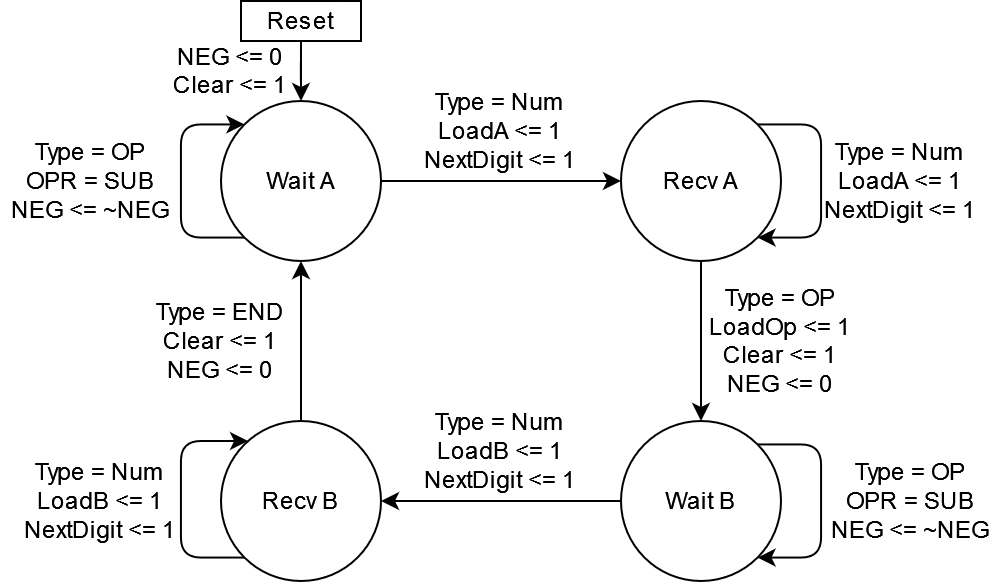
\includegraphics[width=.66\textwidth]{DecoderSM.drawio.png}
    \caption{ASCII Decoder Mealy State Machine Diagram}
    \label{fig:decodersm}
\end{figure} 

Now that the incoming data is understood by the decoder the single numerals and operator need to be interpreted properly, this is done with the state machine in figure \ref{fig:decodersm}.
The state machine will check for its transition conditions anytime any of the inputs change. 
In its initial state, Wait for A, it will wait to receive either valid numeral or the negative operator. 
With the latter the SM will mark the upcoming value as negative, this can occur multiple times meaning that $---1$ will be correctly interpreter as $-1$.
Once a number is received it will be sent to the digit to number converter and the state machine will transition to the Receiving A state. 
In this state the machine checks for new numerals, which will be sent to the converter, and any operation which will mark the end of number A.
This operation will be loaded into a register before the state transitions to the Waiting for B state.
The Waiting for B and Receiving B state mirror the A states, however instead of looking for an operation to mark the end of number B the carriage return is awaited.
The digit to number converter stores the current value, which starts at 0, and upon receiving a new number will multiple the current value by 10 then add the new number. 
\textbf{DOES OVERFLOW CHECKING NEED TO BE ADDED (YES)} 
This new value is then turned if the state machine outputs the negative signal and output to both the A and B registers.
The registers however will only load when the state machine outputs the load A or load B signal at the end of Receiving A and Receiving B states,
these load signals will also clear the converter's current value to allow it to convert the next series of numerals.
Finally when the state machine moves from Receiving B back to Waiting for A it will output a ready signal, indicating that register A, B, and Op contain all the data that needs to be computed.

To achieve this conversion the numeric STD library is utilized both in the decoder with the ASCII data and in the converter turning numerals into larger integers.
%As mentioned maximum size of the incoming integers can be altered with generics, however for the final presented implementation signed 16-bit integers were used.
\subsection{Calculator}

Despite describing this project as a calculator, the calculating component is one of the simplest.
This is due to heavy usage of the numeric STD library which implements the logic required for adding, subtracting, multiplying, and dividing integers.
Furthermore as UART communication is orders of magnitude slower than the clock frequency (115.2 kHz vs 50 MHz)
the speed of even the slowest calculations appears near instant compared to communication (this can be seen on the simulation graph in figure \ref{fig:sim}).

The calculator takes in 2 integers, an operation and ready signal as an input, which it uses to produce a result integer as well as a signal indicating that the calculator is done and a signal indicating an invalid operations, specially dividing by zero or exceeding the signed integer limit.
The current implementation of the calculator is state machine driven, see figure \ref{fig:calcsm}. 
Upon being informed that the data and operation is ready in the registers the machine will send a start signal to the approptatei sub-module for each operations.
Then it will wait for the component to send a ready signal at which point the calculator will forward the result and invalid line from the sub-module to the next component along with a done signal.

\begin{figure}[H]        
    \centering
    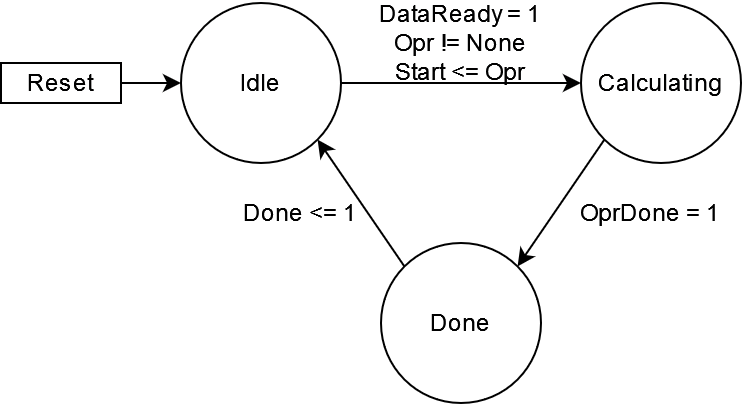
\includegraphics[width=.66\textwidth]{CalculatorSM.drawio.png}
    \caption{ASCII Calculator Mealy State Machine Diagram}
    \label{fig:calcsm}
\end{figure} 

Each of the sub-modules are similar in design, awaiting a start signal which will trigger the operation to begin.
Before and after the operation some error checking is done,
this checking is specific to each modules with the divider checking for divide by zero errors and the other checking if the new output is below the minimum value or above the maximum value.
Once the result is done, valid or invalid, the sub-module will output a done signal.

This approach is rather space inefficient, as each module is independent and shares no components with other components.
As two operations will never occur simultaneously this could be made more efficient,
but the current design is simpler and allows for easy expansion such as adding a exponent function.

\subsection{ASCII Encoder}

Once an integer result is calculated it needs to be converted back into a series ASCII characters and sent out one by one to the UART transmitter.
This is done in the ASCII Encoder and Sender.
This components takes in the signed 16-bit integer results and a done signal from the calculator, and the transmitter's ready signal.
These two stages happen sequentially meaning that a simple state machine is used to control the encoder, shown in figure \ref{fig:encodersm}

% \begin{figure}[H]        
%    \centering
%    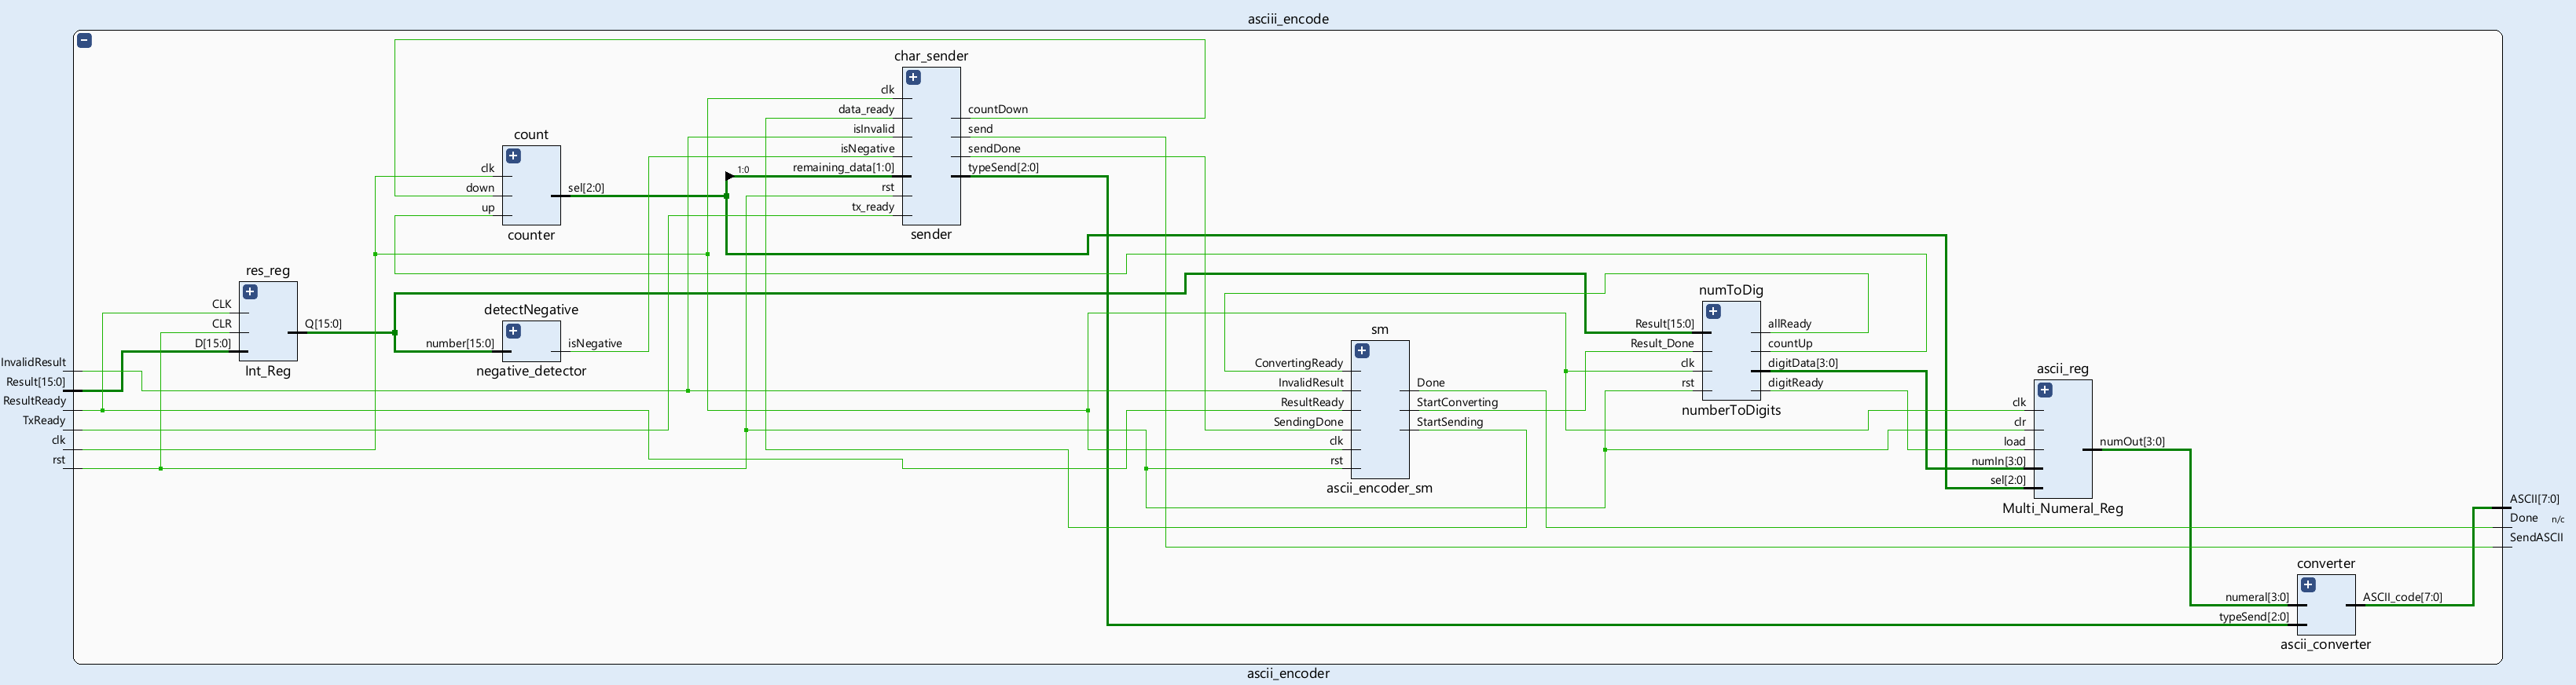
\includegraphics[width=\textwidth]{EncodeImp.png}
%    \caption{ASCII Encoder Block Diagram}
%    \label{fig:encoderimp}
% \end{figure} 

\begin{figure}[H]        
    \centering
    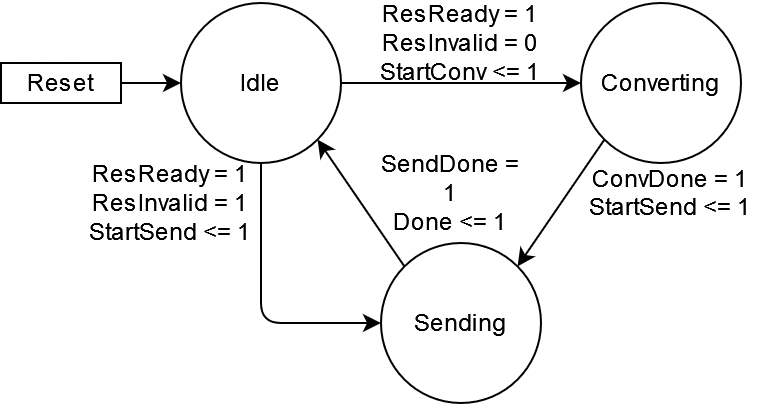
\includegraphics[width=.66\textwidth]{EncoderSM.drawio.png}
    \caption{ASCII Encoder Mealy State Machine Diagram}
    \label{fig:encodersm}
\end{figure} 

When the result is ready the state will transition to converting if the result is valid or go straight to sending if the result is invalid.
Converting from numbers back to digits is a little bit more challenging than the inverse as rather than storing one number multiple numerals need to be stored.
To achieve this there are enough registers to store every digits of the largest possible numbers,
this is done automatically using a log10 and ceiling function at synthesis.
In the case of the signed 16-bit number the largest value is 32767, so 5 registers are required.
The loading of these register is achieved using number to digit converter and a counter.
The converter starts by taking the remainder of result where it divided by ten and then dividing the result by 10.
This remainder is then stored in the register with the index of the counters output. 
Finally if the newly divided result can be divided by 10 again, and not be zero, the counter is incremented and the process starts again.
Following this process means that any number will have its digits stored in the registers, as 4-bit values, with the counter pointing at the highest order term.
This process is identical for both negative and positive values, as the only difference will be wether a negative sign is sent, which will be handled by the sender.
Once this is done a ready signal is sent and the overall state machine will move to the sender.

\subsubsection{Sender}
\begin{figure}[H]        
    \centering
    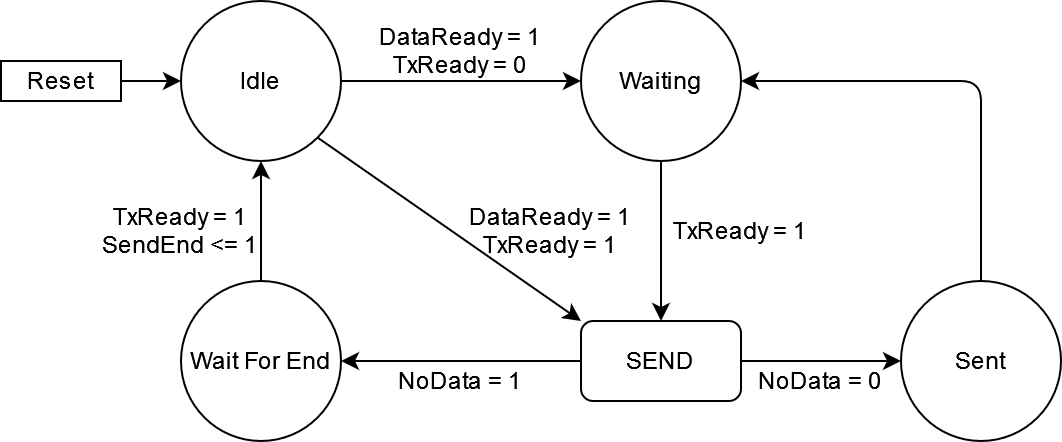
\includegraphics[width=.66\textwidth]{SenderSM.drawio.png}
    \caption{ASCII Sender Mealy State Machine Diagram}
    \label{fig:sendersm}
\end{figure} 

The sender sub-component start after the number has been converted to digits, or immediately upon receiving an invalid number. 
It however shares the digit registers and counters as it will use them for the transmitting.
The sender operators using the state machine in figure \ref{fig:sendersm} as well as an ascii converter which will take numerals and convert them to 8-bit ASCII characters.
Once the data and the transmitter are ready the state machine will send a value, which is a somewhat complicated operation,
then it will wait for the transmitter to be ready either to send the next numeral or, if there is no more data left, it will wait for the carriage return signal to be sent before retuning to idle
The send operation does the following: firstly if the number is negative it will tell the converter to output the ASCII code for a negative sign, number 45, then mark the fact a negative has been sent to avoid repeating this.
Next it will send the numeral to the converter, which will add 48 to the number to make it the ASCII code, and then checks if the counter is at zero.
If the counter is already at zero, it means the number is done sending which is sorted as a variable, otherwise the counter is simply decremented by one.
The exception to all this is if the invalid result input is given, in this case the sender will tell the converter to output the invalid result character (! or ASCII 33) and the end of data variable is set to true.
Then on the final send, when the end of data is true it will tell the converter to output a carriage return and then signal to the state machine that the message is done.
This is the slowest of the components, as for each send a full UART message needs to be sent which is far slower than the clock.

\subsection{Test Bench}

The test bench for simulating the full calculator is identical to the test bench for the UART components.
Once more the test bench creates an instance of the top level implementation in figure \ref{fig:toplevel}
and then creates a second UART components with its own clock to transmit the input and decode the output.
The data for the transmitter is once more a loop that goes through a file with hex codes that will be sent as soon as the transmitter is ready.

Various files were then created to test various scenarios such as dividing by zero and going over the limit.
Figure \ref{fig:sim} shows the calculator computing 1 + 1.
As can be seen in this figure most of the time is spend on receiving and sending, both of which take \textbf{!!!} ns.
Meanwhile calculating form receiving the carriage return to the start of sending the result takes only \textbf{!!!} ns.

\begin{figure}[H]        
    \centering
    
\includegraphics[width=\textwidth]{Logo.png}
    \caption{Simulation of 1 + 1}
    \label{fig:sim}
\end{figure} 

Unlike the multipler before testing all possible inputs is near impossible, as there are $2^{16}$ possible values for A and B, along side for operations meaning that there are $2^{34}$ valid inputs.
This does not including testing more inputs such as injecting random charchater or using more negative signs than nessecary.

Therefor testing was done by \textbf{WE DO NOT HAVE A TESTING STATEGY}


\section{Implementation}

Taking the calculator from design to running on physical hardware posed various challengs.
Firstly was converting all the design to work nicly with-in the provided code for implmentation, such as setting up the proper connections and getting rid of the now obsolete DIP switch connection.
After this various timing issues created problems for the design, all of which were flagged by Vivado. 

\subsection{Timing}

\pagebreak
\printbibliography

\end{document}